\pgfplotsset{compat=1.15}
\usetikzlibrary{arrows}
\usetikzlibrary{positioning}
\definecolor{cqcqcq}{rgb}{0.7529411764705882,0.7529411764705882,0.7529411764705882}
\definecolor{ffzzqq}{rgb}{1,0.6,0}
\definecolor{qqttcc}{rgb}{0,0.2,0.8}
\definecolor{ffqqtt}{rgb}{1,0,0.2}
\definecolor{ffttww}{rgb}{1,0.2,0.4}
\definecolor{ududff}{rgb}{0.30196078431372547,0.30196078431372547,1}
\definecolor{qqwuqq}{rgb}{0,0.39215686274509803,0}
\definecolor{aqaqaq}{rgb}{0.6274509803921569,0.6274509803921569,0.6274509803921569}
\definecolor{uuuuuu}{rgb}{0.26666666666666666,0.26666666666666666,0.26666666666666666}

\begin{figure}
    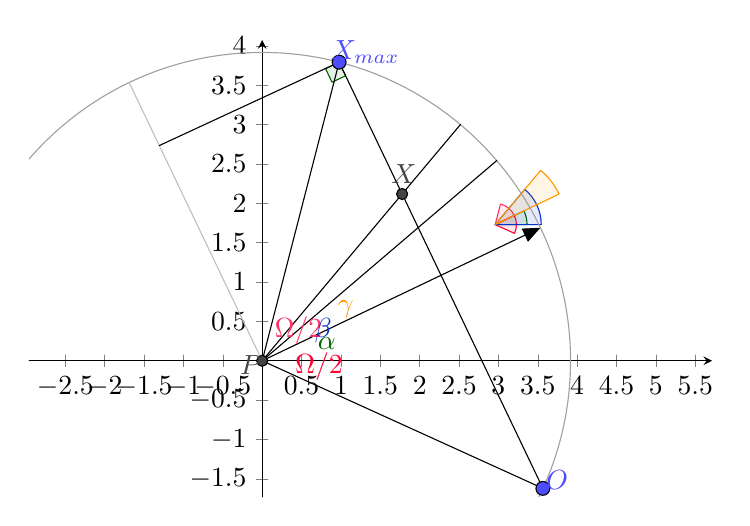
\begin{tikzpicture}[line cap=round,line join=round,>=triangle 45,x=1cm,y=1cm]
        \begin{axis}[
                x=1cm,y=1cm,
                axis lines=middle,
                xmin=-2.958814869512668,
                xmax=5.714480898696139,
                ymin=-1.7293229255592968,
                ymax=4.073867707733968,
                xtick={-2.5,-2,...,5.5},
                ytick={-1.5,-1,...,4},]
            \clip(-2.958814869512668,-1.7293229255592968) rectangle (5.714480898696139,4.073867707733968);
            \draw [shift={(0,0)},line width=0.4pt,color=qqwuqq,fill=qqwuqq,fill opacity=0.10000000149011612] (0,0) -- (0:0.40487376511348167) arc (0:25.552322717163296:0.40487376511348167) -- cycle;
            \draw [shift={(0,0)},line width=0.4pt,color=ffttww,fill=ffttww,fill opacity=0.1] (0,0) -- (25.552322717163293:0.2699158434089878) arc (25.552322717163293:75.55232271716328:0.2699158434089878) -- cycle;
            \draw [shift={(0,0)},line width=0.4pt,color=ffqqtt,fill=ffqqtt,fill opacity=0.1] (0,0) -- (-24.447677282836704:0.2699158434089878) arc (-24.447677282836704:25.55232271716329:0.2699158434089878) -- cycle;
            \draw [shift={(0,0)},line width=0.4pt,color=qqttcc,fill=qqttcc,fill opacity=0.1] (0,0) -- (0:0.5848176607194735) arc (0:50:0.5848176607194735) -- cycle;
            \draw [shift={(0,0)},line width=0.4pt,color=ffzzqq,fill=ffzzqq,fill opacity=0.1] (0,0) -- (25.552322717163293:0.8997194780299592) arc (25.552322717163293:50:0.8997194780299592) -- cycle;
            \draw[line width=0.4pt,color=qqwuqq,fill=qqwuqq,fill opacity=0.10000000149011612] (0.8047870042229275,3.7096540754257243) -- (0.8871113412093425,3.5374623659814546) -- (1.059303050653612,3.6197867029678696) -- (0.976978713667197,3.7919784124121394) -- cycle;
            \draw [line width=0.4pt,color=aqaqaq] (0,0) circle (3.915812519408775cm);
            \draw [->,line width=0.4pt] (0,0) -- (3.532813803328211,1.6890276250470742);
            \draw [line width=0.4pt] (0,0)-- (2.517035769331392,2.999686420788817);
            \draw [line width=0.4pt] (0,0)-- (2.97834267549334,2.5422554148813745);
            \draw [line width=0.4pt,color=cqcqcq] (-1.6890276250470742,3.532813803328211)-- (0,0);
            \draw [line width=0.4pt] (0.976978713667197,3.7919784124121394)-- (-1.306662686194439,2.733049421825162);
            \draw [line width=0.4pt] (0.976978713667197,3.7919784124121394)-- (0,0)-- (3.5647191665507085,-1.6206063528150567);
            \draw [line width=0.4pt] (0.976978713667197,3.7919784124121394)-- (3.5647191665507085,-1.6206063528150567);
            \begin{scriptsize}
                \draw [fill=uuuuuu] (0,0) circle (2pt);
                \draw[color=uuuuuu] (-0.14269290327889572,-0.051346099033414735) node {$P$};
                \draw[color=qqwuqq] (0.8200069382131606,0.21856974437557433) node {$\alpha$};
                \draw [fill=ududff] (0.976978713667197,3.7919784124121394) circle (2.5pt);
                \draw[color=ududff] (1.3103540537394884,3.9254139938590242) node {$X_{max}$};
                \draw[color=ffttww] (0.46011914700117695,0.38951644520126744) node {$\Omega$/2};
                \draw [fill=ududff] (3.5647191665507085,-1.6206063528150567) circle (2.5pt);
                \draw[color=ududff] (3.744095241810528,-1.5088916534419556) node {$O$};
                \draw[color=ffqqtt] (0.7210377956298651,-0.069340488594014) node {$\Omega$/2};
                \draw[color=qqttcc] (0.7750209643116626,0.3805192504209678) node {$\beta$};
                \draw[color=ffzzqq] (1.0629311972812496,0.6504350938299569) node {$\gamma$};
                \draw [fill=uuuuuu] (1.7772701770007864,2.118068118451234) circle (2pt);
                \draw[color=uuuuuu] (1.8007011692658161,2.368899296867187) node {$X$};
            \end{scriptsize}
        \end{axis}
    \end{tikzpicture}
    \label{fig:raycasting}
    \caption{Raycasting}
\end{figure}
